%%%%%%%%%%%%%%%%%%%%%%%%%%%%%%%%%%%%%%%%%%%%%%%%%%%%%%%%%%%%%%%%%%%%%%%%%%%%%%%%%
%
% Purpose:  Mathematical Formulation part of Product Spec for the ThermalRider model
%
% 
%
%%%%%%%%%%%%%%%%%%%%%%%%%%%%%%%%%%%%%%%%%%%%%%%%%%%%%%%%%%%%%%%%%%%%%%%%%%%%%%%%

\section{Mathematical Formulations}

\subsection{Basic Equations}

The equation for temperature of a facet is based on an emission-absorption
model.  Thermal emission is modeled using a black-body baseline, modified by the
emissivity of the surface.  The total power, $P$, radiated by a surface
at temperature $T$ and with surface area $A$ is 

\begin{equation}\label{eqn:thermalemission}
P = \epsilon \sigma A T^4 
\end{equation}

where $\epsilon$ is the emissivity of the surface, 
and $\sigma$ is the Stefan-Boltzmann constant, $\sigma = 5.6704004 \times
10^{-8} \ W \; m^{-2} \; K^{-4}$

We model the power absorbed $P_{abs}$ as the sum of the power from external
sources of radiation, thermal input from the vehicle, and as a possible future
extension, conduction from other facets.  The current implementation ignores
conduction.

The net flow of power can be represented as a rate of change of temperature by
factoring in the specific heat of the facet,

\begin{equation}\label{eqn:temperatureODE}
Q \frac{dT}{dt} = P_{abs} - \epsilon \sigma A T^4
\end{equation}

where $Q$ is the specific heat, expressed in  $J \cdot K^{-1}$
and $P_{abs}$is the rate at which energy 
is absorbed into a facet.

\subsection {Temperature Propagation}

 The conventional JEOD approach to solving ~\ref{eqn:temperatureODE} has been
to use a special $4^{th}$ order Runge-Kutta technique which is included in the 
\textit{ThermalFacetRider} class.  This technique includes a series of tests
in order to avoid instabilities resulting from an integration step too large
to accommodate rapidly varying temperatures.

With the introduction of first order methods in the \textit{er7\_utils} package,
it is now possible to have JEOD propagate temperature just as it propagates
the state of a vehicle.  This approach required the introduction of the 
new \textit{ThermalIntegrableObject} class which is derived from
\textit{er7\_utils::IntegrableObject}.  The \textit{integrate} method of
\textit{ThermalIntegrableObject} performs each step of the integration cycle.
This method also checks at each step to make sure that the
equilibrium temperature is not surpassed within an integration cycle.

\subsection{Runge-Kutta 4th Order (RK4) Integrator}\label{ref:thermalRK4integrator}

The rate at which temperature changes is a strong function of
temperature due to the rate of thermal emission, as described 
in equation \ref{eqn:thermalemission}.
It is assumed that other contributing factors change more slowly, 
indeed that they are constant over an integration step.
All other factors are combined into the value \textit{power\_absorb}, which 
is positive if there is a net power into the facet (excluding thermal emission), and negative if there is a net flow out from the surface 
(e.g. from a thermal source within the vehicle).
With those assumptions, the RK4 integrator can be implemented as follows:

$T_0$ represents the initial temperature at the start of the integration step.

The first full-step approximation to the temperature change, $I_1$, is
calculated as 
\begin{equation*}
I_1 = \frac{\Delta t}{Q} \left(  P_{abs} - \epsilon \sigma A T_0^4 \right)
\end{equation*}

The second step uses the mid-point temperature as the operating temperature, calculated as the average of $T_0$ and $T_0 + I_1$.   
\begin{equation*}
T_1 = T_0 + \frac{I_1}{2}
\end{equation*}
\begin{equation*}
I_2 = \frac{\Delta t}{Q} \left(  P_{abs} - \epsilon \sigma A \left(T_1 \right) ^4 \right)
\end{equation*}

The third step uses the mid-point temperature, calculated as the
average of $T_0$ and $T_0 + I_2$ as the operating temperature,  
\begin{equation*}
T_2 = T_0 + \frac{I_2}{2}
\end{equation*}
\begin{equation*}
I_3 = \frac{\Delta t}{Q} \left(  P_{abs} - \epsilon \sigma A \left(T_2 \right) ^4 \right)
\end{equation*}

The  fourth step uses the predicted end value, $T_0 + I_3$ as the
operating temperature,  
\begin{equation*}
T_3 = T_0 + I_3
\end{equation*}
\begin{equation*}
I_4 = \frac{\Delta t}{Q} \left(  P_{abs} - \epsilon \sigma A \left(T_3 \right) ^4 \right)
\end{equation*}

The actual change in temperature is then calculated as a weighted average of those 4 values,
\begin{equation*}
\Delta T = \frac{I_1+2I_2+2I_3+I_4}{6}
\end{equation*}

\subsubsection{Integrating close to the asymptote}
If the integration time-step is large compared to the characteristic time over
which the temperature can change appreciably, there is the potential that the
RK4 integrator can become unstable.  This is due to the asymptotic nature of the
temperature$\sim$time evolution; whether the temperature is above or below the
equilibrium temperature, the temperature will asymptotically approach equilibrium.  The instability is observed when the integration time-step is
sufficiently large that the local
linearization of that asymptotic approach jumps over the asymptote in one step,
and then tries to approach from the other side.

Figure \ref{fig:tempasymptote} illustrates the temperature$\sim$time profile, with the asymptotic trend both above and below the asymptote at $T_{eq}$.  Note that the two profiles are not symmetric; the upper profile is a little steeper for the same temperature difference from $T_{eq}$, making this instability more likely when approaching from above than when approaching from below.


\begin{figure}[htp]
\begin{center}
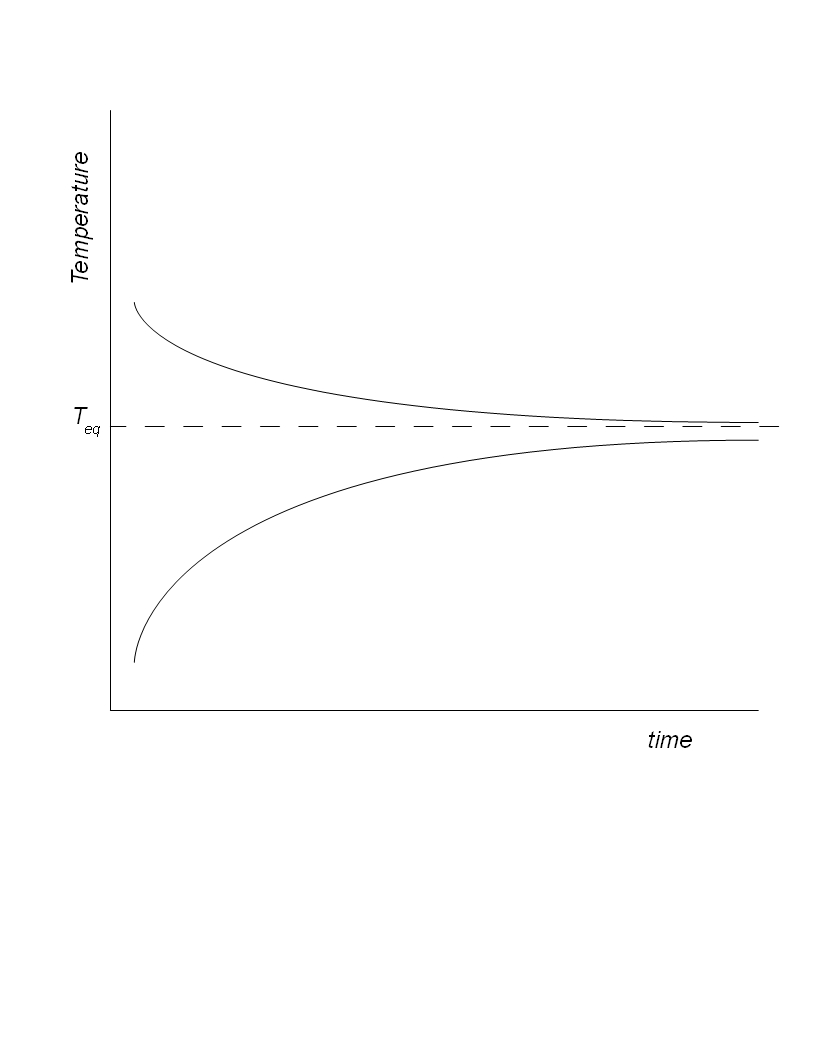
\includegraphics[width=3.2736in,height=2.85in]{figures/temp_integ.jpg}
\caption{Illustration of the temperature$\sim$time profile near the equilibrium temperature.}
\label{fig:tempasymptote}
\end{center}
\end{figure}

\begin{quotation}
Aside:  The rate at which the surface radiates energy is $P_{rad} \propto T^4$.

The rate at which the surface absorbs energy is some constant $P_{abs}$.  

At equilibrium, these two are equivalent,  $P_{abs} = P_{rad} \propto {T_{eq}}^4$.


The net rate at which energy increases is therefore
\begin{equation*}
\epsilon = (P_{abs} - P_{rad}) \propto \frac{dT}{dt}.
\end{equation*}  

Therefore, 
\begin{equation*}
\frac{dT}{dt} \propto ({T_{eq}}^4 - T^4).
\end{equation*}  

Then for some deviation from the equilibrium temperature:
\begin{equation*}
T=T_{eq}+\Delta T \Rightarrow \frac{dT}{dt} \propto 
(-) \left( T_{eq} \right)^4 
\left(
4 \left( \frac{\Delta T}{T_{eq}} \right) + 
6 \left( \frac{\Delta T}{T_{eq}} \right)^2 + 
4 \left( \frac{\Delta T}{T_{eq}} \right)^3 + 
  \left( \frac{\Delta T}{T_{eq}} \right)^4 
\right)
\end{equation*}  

The difference between above the asymptote and below the asymptote results from the sign change on $\Delta T$.  The first and third terms will have different signs for the two cases, whereas the second and fourth will have the same sign regardless of whether the temperature is above or below the asymptote.  The consequence is that above the asymptote, all terms are additive, and below the asymptote the terms tend to cancel each other.

\end{quotation}

Figure \ref{fig:tempasymptote1} illustrates the problem with having an
integration time-step that is too large.  In the first step, the original
temperature ($T_0$) is used to calculate the rate of change of temperature, and
the predicted change to that temperature ($I_1$).  Next, that change is used to
derive an intermediate temperature ($T_1 = T_0 + 0.5 I_1$), which is below the
asymptote.  This temperature is used to calculate a new temperature gradient
which is now positive; that temperature gradient is used to calculate a new
correction ($I_2$, not shown) to the original temperature.  The next
intermediate temperature ($T_2 = T_0 + 0.5 I_2$) will then be higher than $T_0$,
therefore have a steeper gradient, which leads to $I_3$ having a larger
deviation than did $I_1$.  Thus, the calculation of $T_3 = T_0 + I_3$ falls far
below the equilibrium value, which is highly erroneous, and further leads to a
ridiculously large value for $I_4$.  The consequence is that the temperature
change could be driven to non-physical values, and in the opposite direction to which it should have been evolving.

\begin{figure}[htp]
\begin{center}
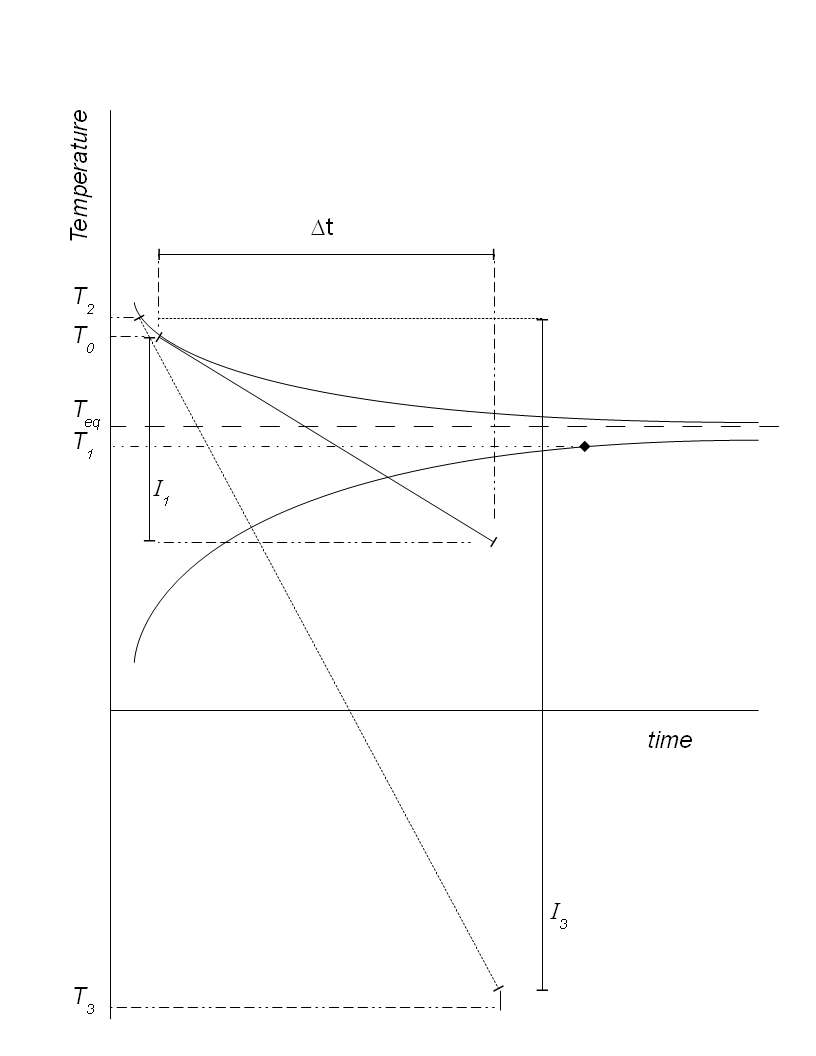
\includegraphics[height=200mm]{figures/temp_integ1.jpg}
\caption{Illustration of the instability near the equilibrium temperature.}
\label{fig:tempasymptote1}
\end{center}
\end{figure}

To prevent this instability, there are numerous checks made during the integration.  First, the direction of anticipated temperature change is recorded as \textit{dt\_dir} ($\pm 1$ corresponding to up and down) by comparing the original temperature to the equilibrium temperature.

Next, $I_1$ is calculated; it is assumed that $I_1$ has the correct direction to it.  $I_1$ is used to calculate $T_1$ and thereby $I_2$, the latter of which is compared against \textit{dt\_dir} to ensure that it is in the correct direction.  If this is not the case, the predicted temperature is set to the equilibrium temperature and the integration ends.

The same check could be made on $I_3$, but it is not necessary.  Since $T_1$ is closer than $T_0$ to $T_{eq}$, the magnitude of $I_2$ must be less than the magnitude of $I_1$.  Therefore, if $I_1$ was insufficient to cross the asymptote, $I_2$ must have been likewise; hence if $I_2$ was in the correct direction, $I_3$ must also be in the correct direction.

The same is not true of $I_4$, since $T_3$ uses a full-step correction to $T_0$, whereas $T_1$ and $T_2$ used only half-step corrections.  $T_3$ could, therefore, be on the wrong side of the equilibrium temperature.  Incorporating $I_4$ in this situation would lead to a calculated temperature change that is too small; ignoring it would lead to the value being too large, and the final temperature being very close to equilibrium.  Instead, one-half of the value is taken.

The four temperature deviations are combined then to give the final temperature change.

Once again, checks are made that this is sensible.  If the temperature change was in the wrong direction (this may be impossible), or if the temperature change results in a new temperature that is on the wrong side of equilibrium (this, too, may be impossible) the temperature is set to the equilibrium temperature.




\subsection{Emitted Power}
The mean emitted power over the integration step can now be calculated from the resulting change to the temperature.

\begin{equation}
P_{emit} = Q\frac{ \Delta T}{\Delta t} - P_{abs}
\end{equation}

Note: a positive value of $P_{emit}$ means that the facet gains
energy by emission (physically impossible).  $P_{emit}$ is typically negative.
